\documentclass[11pt, oneside]{article}   	% use "amsart" instead of "article" for AMSLaTeX format
\usepackage[margin=1in]{geometry}                		% See geometry.pdf to learn the layout options. There are lots.
\geometry{letterpaper}                   		% ... or a4paper or a5paper or ... 
%\geometry{landscape}                		% Activate for rotated page geometry
\usepackage[parfill]{parskip}    		% Activate to begin paragraphs with an empty line rather than an indent
\usepackage{graphicx}				% Use pdf, png, jpg, or eps§ with pdflatex; use eps in DVI mode
								% TeX will automatically convert eps --> pdf in pdflatex		
\usepackage{amssymb}
\usepackage{etoolbox}
\usepackage{lipsum}
    \AfterEndEnvironment{hangparas}{\addvspace{0.67\baselineskip}}
    \usepackage[notquote]{hanging}


\title{Here's What (and Whom) to Avoid When Driving}
\author{Desmond Cole, Teerth Patel, Yunbin Peng}

\begin{document}
\maketitle
\section*{Introduction}
We analyze traffic fatality data provided by the National Highway Traffic Safety Administration (NHTSA) to assess various predictors of traffic fatalities and develop a limited profile of the circumstances associated with traffic fatalities.

\section*{Exploratory Analysis and Visualization}

\subsection*{Geographic Patterns}

\subsection*{Time Trends}
\textbf{Daily Cycle} \\
At the national and state level, the cycle of fatal accidents throughout the day is fairly consistent. The below plot shows aggregate fatal accidents per thousand vehicles per hour for the United States, between 2015 and 2016. To account for traffic variability, we weighted the rate of fatal incidents according to hour-by-hour traffic flow allocations estimated by Batterman, et al. (see references). These same flow allocations are used to weight state-by-state hourly trends. \\
\\
\begin{center}
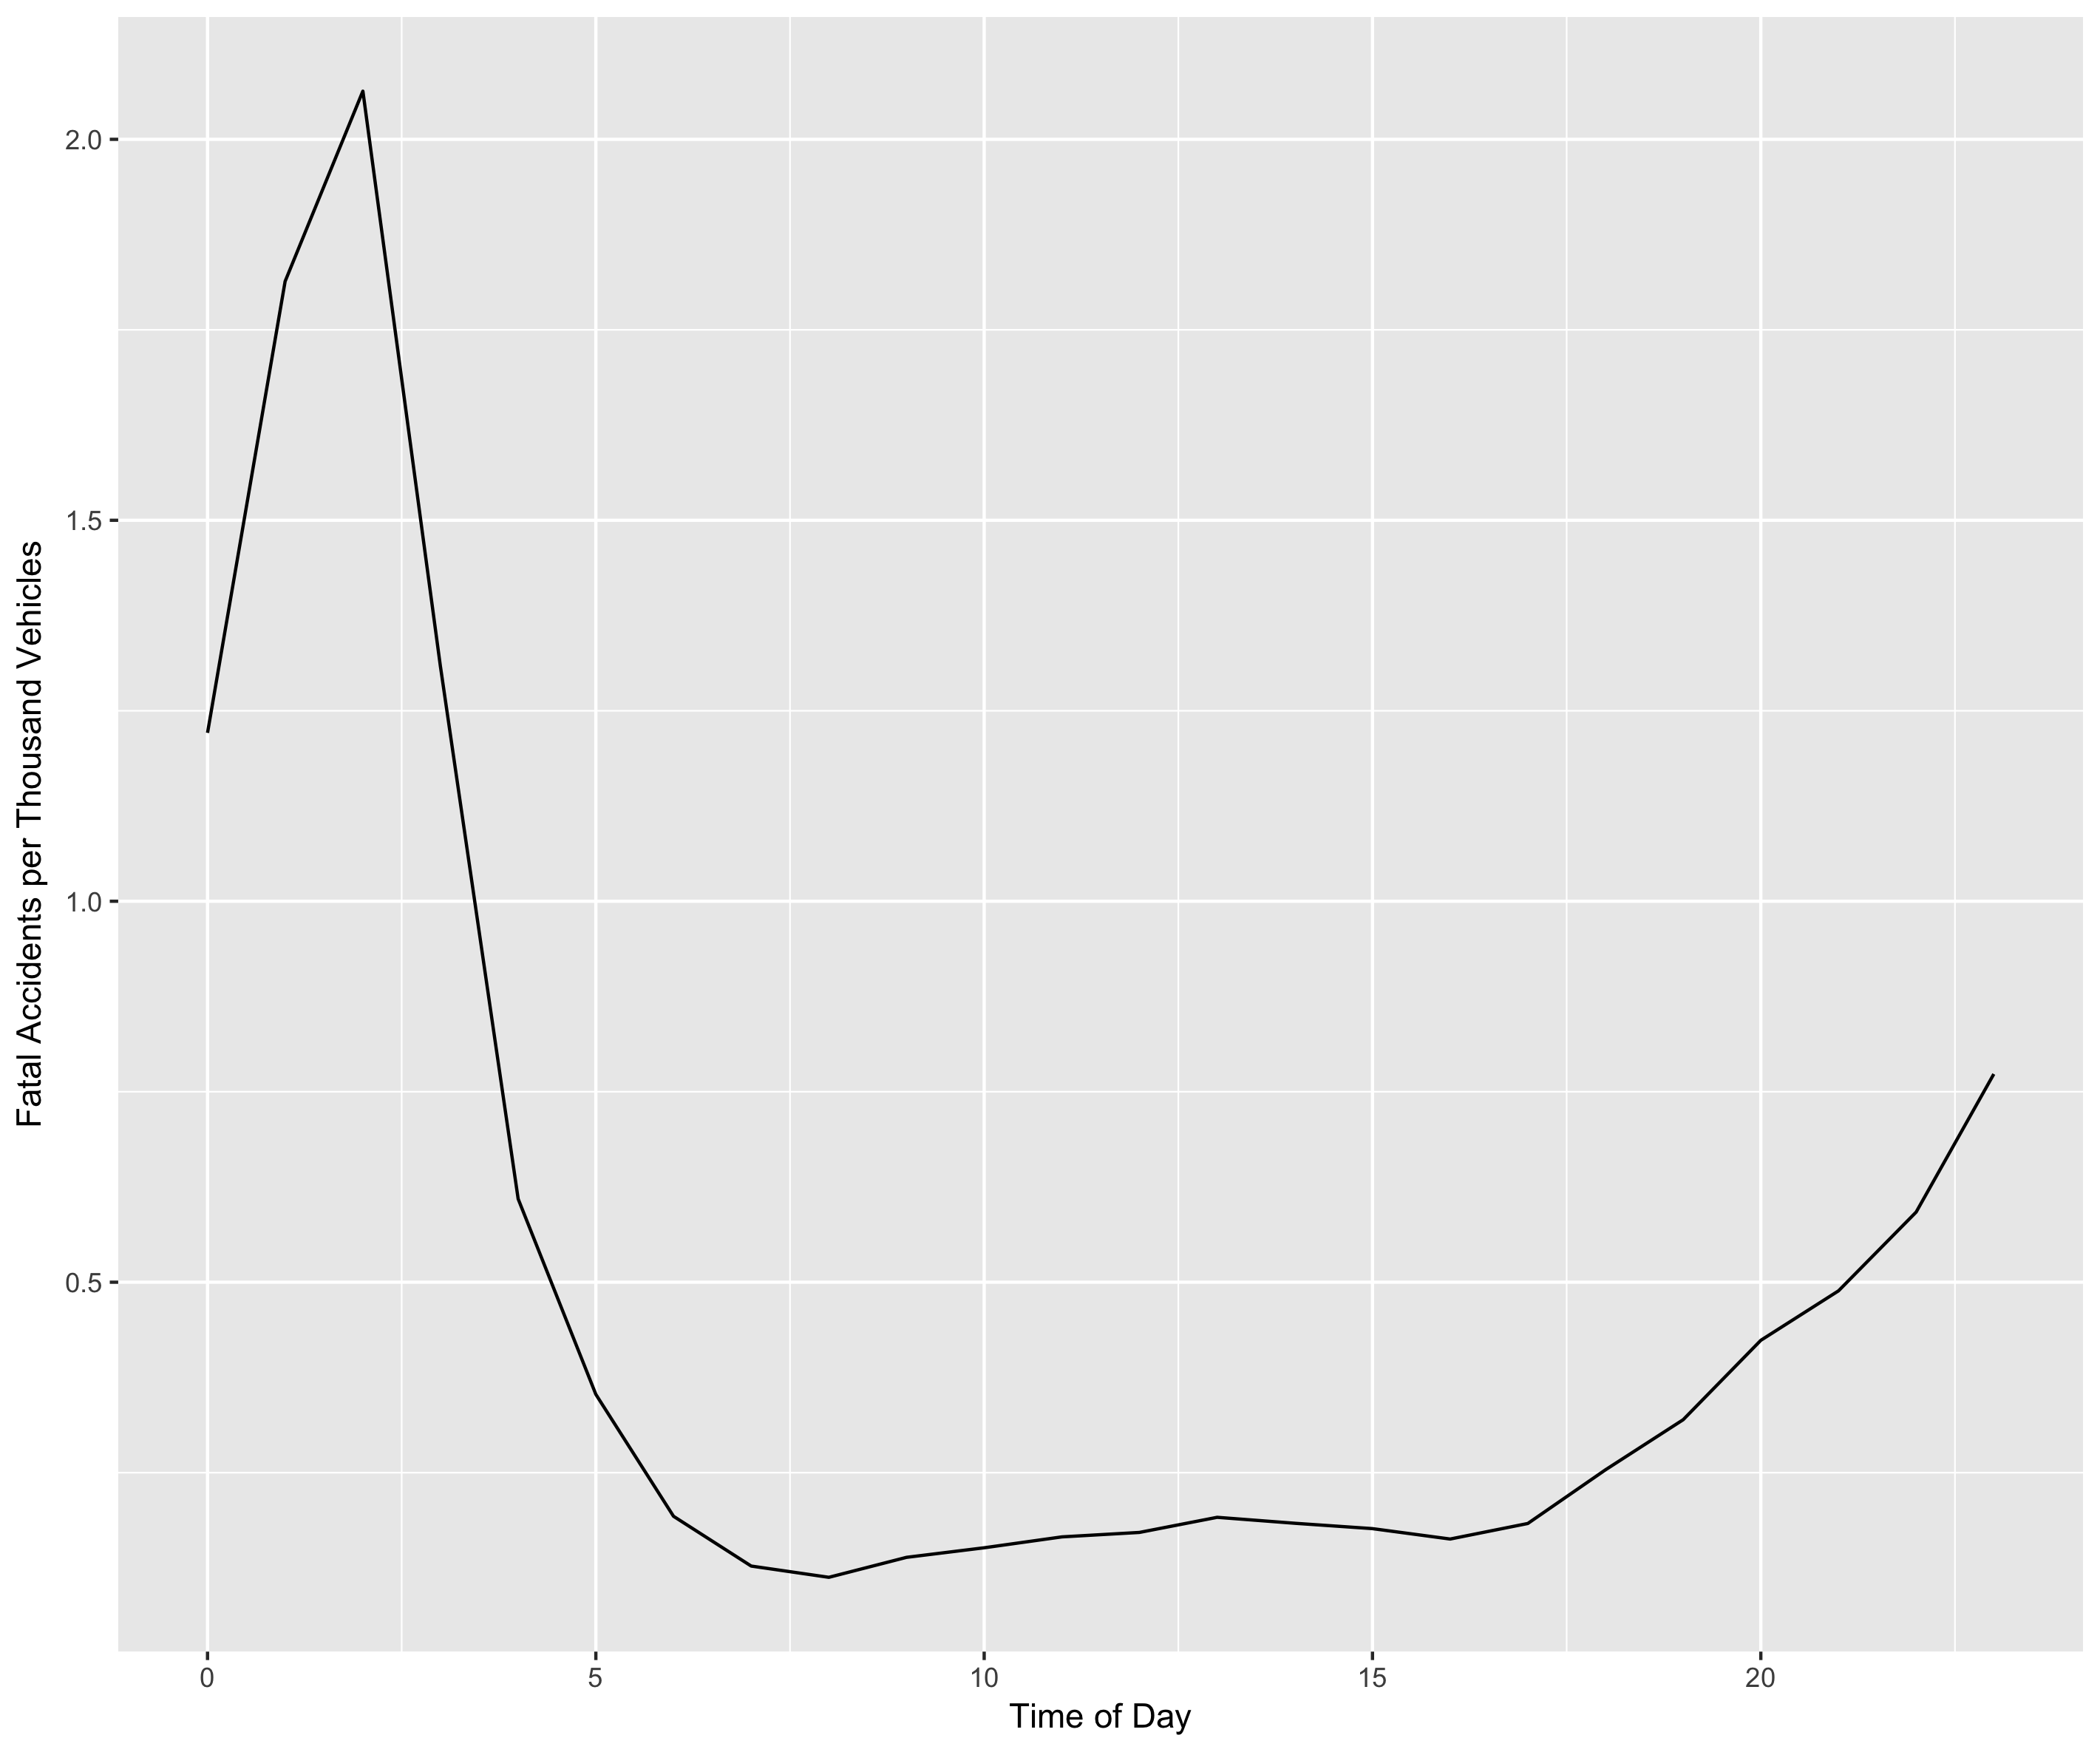
\includegraphics[width=.75\textwidth]{WeightedNationalDayTrends.png}
\end{center}

At the state level, the daily fatal accident cycle is roughly similar. Estimating the overall traffic flow for each state using state-level vehicle registrations, combined with the flow allocations estimated by Batterman, et al. (2015), returns state-level cycles that closely mirror the overall national trend.

\begin{center}
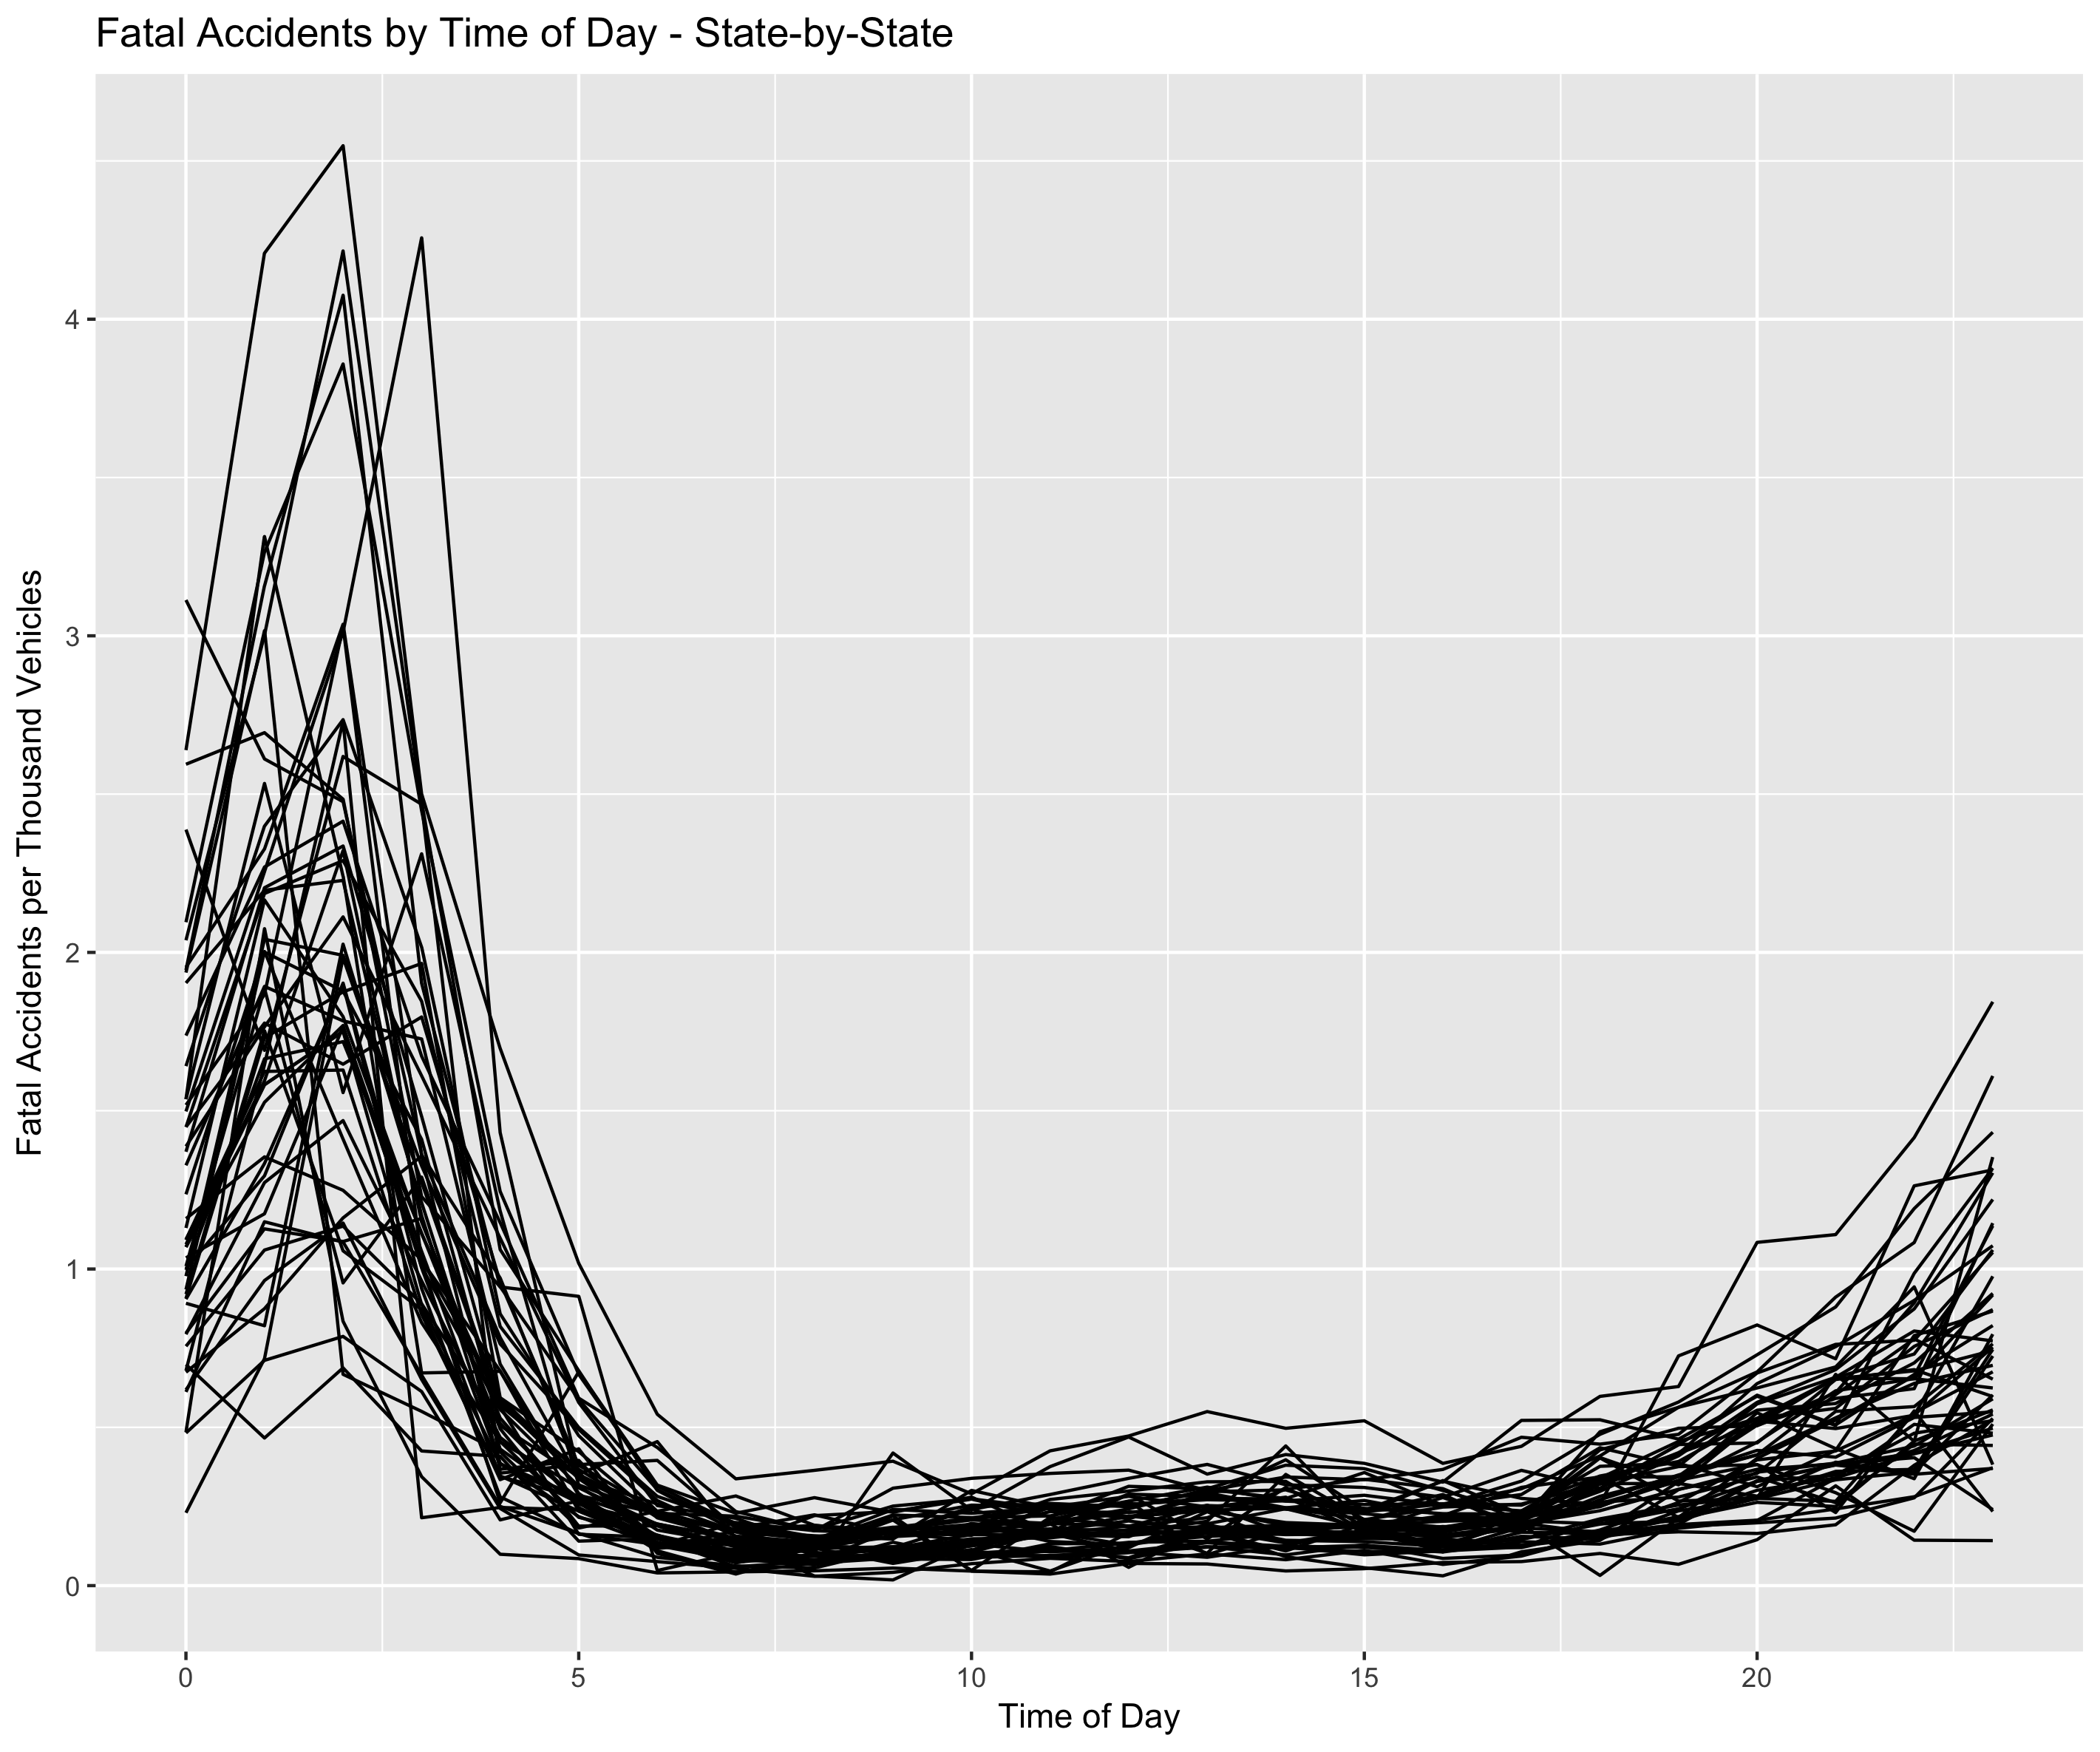
\includegraphics[width=.75\textwidth]{WeightedStatePlot.png}
\end{center}

To tease out any potential state-level variation in daily cycles, we used shape-based time series clustering, available in R's dtwclust package. Roughly speaking, this method clusters different time series based on their similarity to different centroids, where a centroid in this case is defined as a typical time series. Further detail on relevant methods is available in work by Gravano and Paparrizos (2015). Testing several different numbers of clusters yielded little overall diversity in terms of performance. A plot of results obtained using 3 clusters is below. There is little indication of significant variation across clusters, suggesting that hourly fatal incident cycles vary little across the United States.

\begin{center}
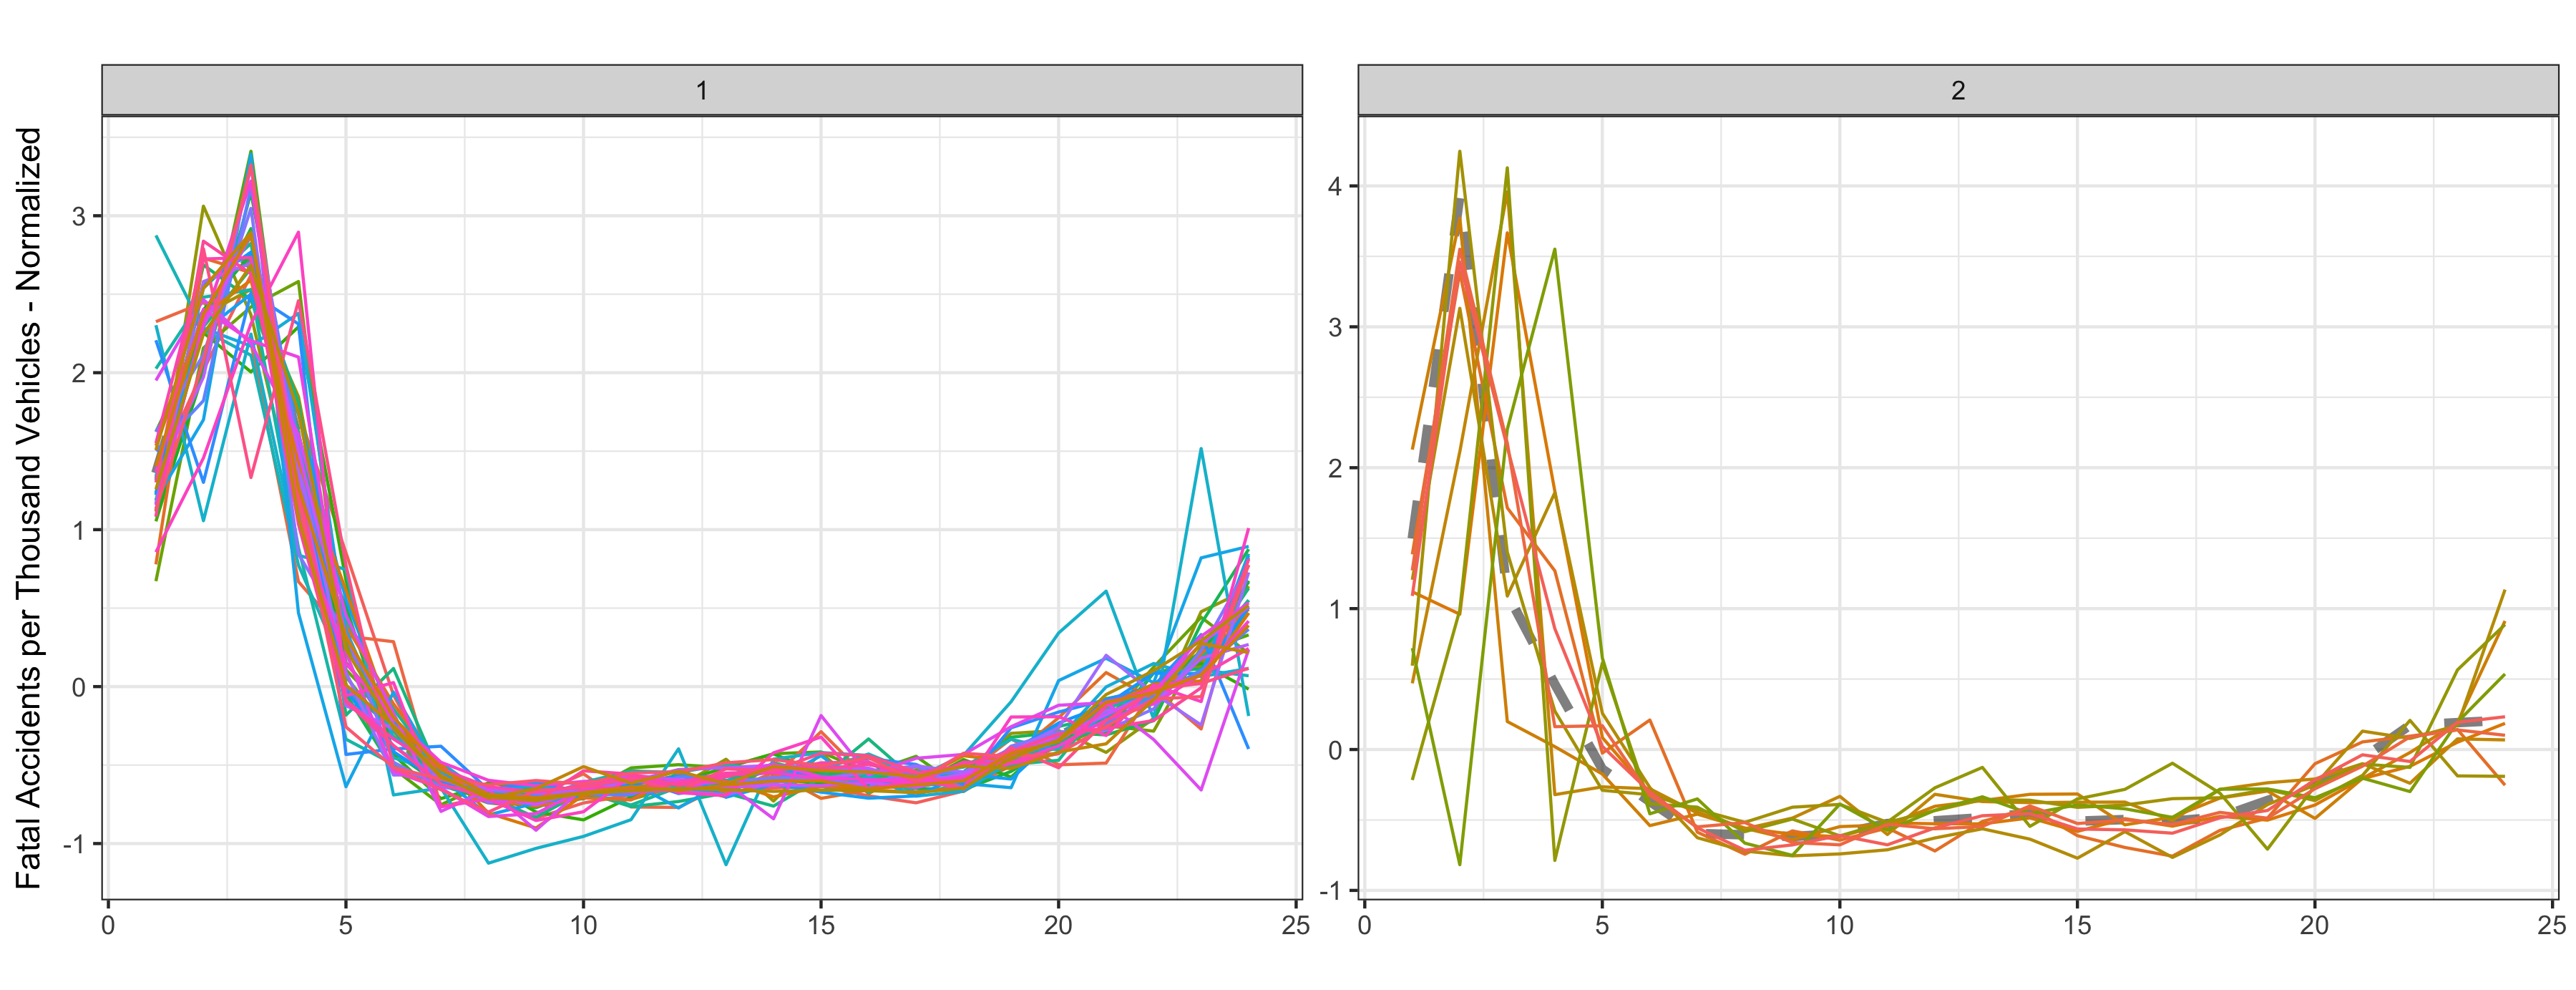
\includegraphics[width=.75\textwidth]{StateClusterPlot_Hourly.png}
\end{center}

(Insert table of clustering performance)

\textbf{Weekly Cycle} \\

\section*{Risks of Traffic Fatalities}
We used a mix of classifiers to assess factors relevant to incident fatalities, with a particular focus on driver behavior and vehicle manufacturer. In many cases, we had to grapple with significant class imbalance. For example, there are far more single-fatality incidents than multi-fatality incidents. As a result, optimal classification in the naive setting without any resampling will occasionally identify all incidents as single-fatality.   

\subsection*{Driver Behavior}
\textbf{Drugs/Alcohol}
\textbf{Distraction}

\subsection*{Automakers}

This section explores in some detail different fatality rates for different car types (by automaker, vehicle body, etc.).\footnote{Note that the numbers in this assessment focus on car brands \textit{involved} in fatal incidents. Thus, they do not imply specifically that the vehicle types considered here actually caused death(s), or that the driver(s) of the vehicle(s) themselves died.} For this assessment, we focused on the 15 largest automakers that together produce more than 95\% of the cars and light trucks on American roads. In addition, we subsetted the data to focus specifically on smaller vehicles, excluding commercial vehicles, semi-trucks, etc. \\

The plot below shows a basic ranking of car manufacturers according to the number of fatalities per million vehicles.

(Insert graph of fatalities/fatal accidents by car manufacturer) \\


The plot above, although suggestive of meaningful difference across manufacturers, fails to fully account for the various contextual differences which may be unobservable. To further explore the relevance of car manufacturer, we consider the relationships between car model and various fatality-related predictors, to understand if a given manufacturers' products tend to be associated with high-risk behaviors or other crash factors. The table below shows the results from various multi-class classifications of car manufacturer ran using a set of crash-relevant predictors .... The results do not suggest any substantial mechanism(s) by which a car's make determines the risk of it being involved in a fatal incident. \\

(Insert table of classifications and results) \\

As an alternative to classification, we applied multidimensional scaling to assess visually the differences between the major automakers in terms of various crash-relevant pieces of information. These results suggest some moderate clustering of driver behavior. BMW and Jaguar-Land Rover, both of which are luxury brands, are spaced relatively far from more truck-oriented manufacturers such as GM and Ford. In addition, Mitsubishi, which as a brand appears to include many heavier-duty vehicles, is an outlier from the majority of the other automakers.\\

(Insert MDS plot) \\



\subsection*{Multi-fatality Incidents}
Another specific category of interest is multi-fatality incidents. Every observation in the available data describes an instance of a given person dying, but what about multiple deaths? To explore this issue, we generated a binary 1-0 indicator for whether an incident involved more than 1 fatality, and tested the classification performance of a series of different models, the results of which are shown below.



\section*{Conclusion}

\section*{References}
\begin{hangparas}{1.27cm}{1}
Batterman, Stuart, Richard Cook, and Thomas Justin. "Temporal variation of traffic on highways and the development of accurate temporal allocation factors for air pollution analyses." \textit{Atmos Environ}. Apr. 2015.

Choi, Eun-Ha. "Crash Factors in Intersection-Related Crashes: An On-Scene Perspective." \textit{U.S. Department of Transportation - National Highway Traffic Safety Administration}. Sept. 2010.

Gravano, Luis and John Paparrizos. "k-Shape: Efficient and Accurate Clustering of Time Series." \textit{SIGMOD}. June 2015.

Zador, P.L, S.A. Krawchuk, and R.B. Voas. "Relative Risk of Fatal Crash Involvement by BAC, Age, and Gender." \textit{U.S. Department of Transportation - National Highway Traffic Safety Administration}. Apr. 2000.




\end{hangparas}




\end{document}  